\documentclass{beamer}

\usepackage{beamerthemesplit}
\usetheme{Copenhagen}

\title{An Overview of Overture}
\author{Miguel Ferriera and Kenneth Lausdahl}
\date{\today}

\begin{document}

\frame{\titlepage}

\section[Outline]{}
\frame{\tableofcontents}

\section{Introduction}
\subsection{Abstract}
\frame
{
  \frametitle{Abstract}

\begin{block}<+->{Abstract}
A short introduction to the Overture project showing how to bootstrap the tools for VDM. Short demo of the Editor and Debug execution.
\end{block}


}


\subsection{Overview of the Overture components}
\frame
{
  \frametitle{Overview of the Overture components}

\begin{figure}[t]
\centering
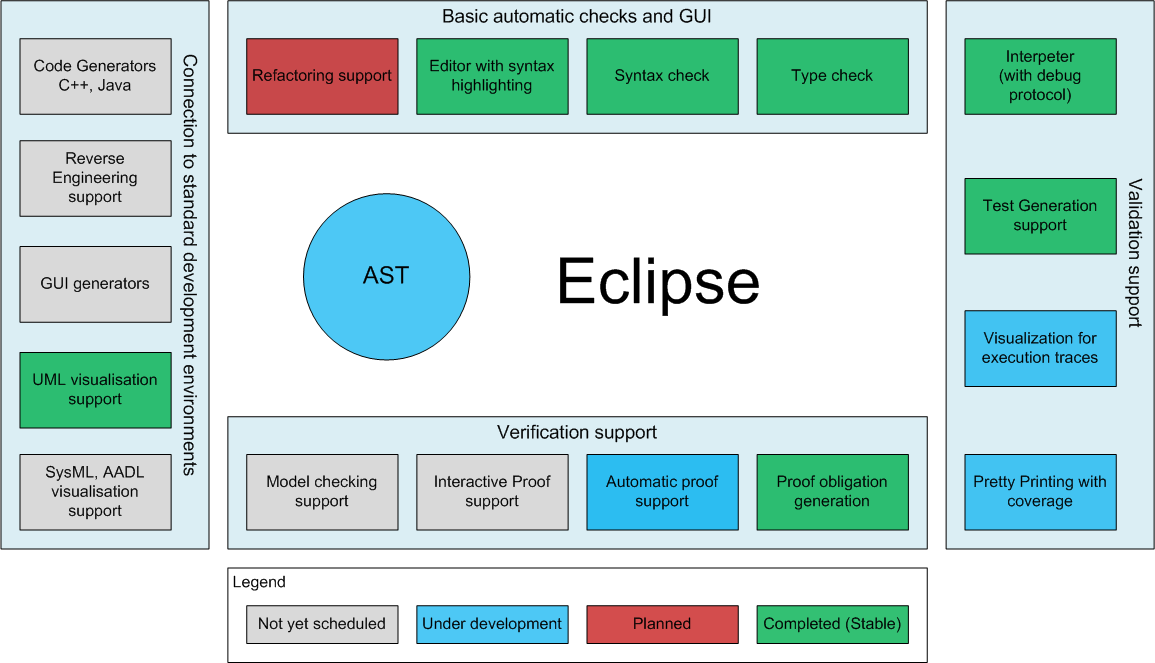
\includegraphics[width=\textwidth]{images/OvertureOverview}
%\caption{}
\label{fig:}
\end{figure}

}

\frame
{
  \frametitle{Overview of the Overture components}
Main component categories:
  \begin{itemize}
  \item<1-> Basic automatic checks and GUI.
  \item<2-> Connections to standard development environments.
  \item<3-> Validation support.      
  \item<4-> Verification support.
  \end{itemize}
}

\frame
{
  \frametitle{Basic automatic checks and GUI}

  \begin{itemize}
  \item<1-> Refactoring support.
  \item<1-> Editor with syntax highlighting.
  \item<1-> Syntax check.      
  \item<1-> Type check.
  \end{itemize}
}

\frame
{
  \frametitle{Connections to standard development environments}

  \begin{itemize}
  \item<1-> Code Generators C++, Java.
  \item<1-> Reverse Engineering support.
  \item<1-> GUI generators.      
  \item<1-> UML visualization support.
  \item<1-> SysML, AADL visualization support.
  \end{itemize}
}

\frame
{
  \frametitle{Validation support}

  \begin{itemize}
  \item<1-> Interpreter (with debug protocol).
  \item<1-> Test generation support.
  \item<1-> Visualization for execution traces.      
  \item<1-> Pretty Printing with coverage.
  \end{itemize}
}

\frame
{
  \frametitle{Verification support}

  \begin{itemize}
  \item<1-> Model checking support.
  \item<1-> Interactive Proof support.
  \item<1-> Automatic proof support.      
  \item<1-> Proof obligation generation.
  \end{itemize}
}


\section{Overture Tools}


\subsection{VDMJ}
\frame
{
  \frametitle{VDMJ}

Supported features
  \begin{itemize}
  \item<1-> Syntax check.      
  \item<1-> Type check.
  \item<1-> Interpreter (with debug protocol).
  \item<1-> Pretty Printing with coverage. (partly)
  \item<1-> Test generation support.
  \item<1-> Proof obligation generation.
% Multi dialect VDM pp sl VICE
  \end{itemize}
}


\subsection{Overture Editor}
\frame
{
  \frametitle{Overture Editor}

Supported features
  \begin{itemize}
  \item<1-> Editor with syntax highlighting.
  \item<1-> Syntax check.      
  \item<1-> Type check.
  \item<1-> UML visualization support.
  \item<1-> Interpreter (with debug protocol).
  \item<1-> Test generation support.
  \end{itemize}
}

\frame
{
  \frametitle{Overture Editor Main view}

 A picture of the editor
}

\frame
{
  \frametitle{Overture Editor Demo}

  \begin{itemize}
  \item<1-> Demo Editor with syntax highlighting, syntax and type check.
  \item<2-> Debug with break points.      

  \end{itemize}
}

\section{About Overture}
\frame
{
  \frametitle{The Overture project}

\begin{block}<+->{Mission}
Overture's mission is twofold: 
  \begin{itemize}
  \item<1-> to provide an industrial-strength tool that supports the use of precise abstract models in software development, and 
  \item<1-> to foster an environment that allows researchers and other interested parties to experiment with modifications and extensions to the tool.      

  \end{itemize}
\end{block}

The Overture tools are being developed by volunteers, research scientists and students. See more at:
\begin{center}
\href{www.overturetool.org}{www.overturetool.org}
\end{center}

}



\end{document}
